\subsection{Relating DOM Changes to the Application's Code} \label{Sec:domToCode}
%\IncMargin{0em}
\begin{algorithm}[t]
{\scriptsize
\SetKwInOut{Input}{input}\SetKwInOut{Output}{output}
\Input{Test suite $T$; The set of test cases $tc_i \in T$}
\Output{The ordered set of oracles $oracles$}
\BlankLine

\Begin {
\nl \For{$tc_i \in T$}{
\nl  $trace \leftarrow textsc{Exec}(tc_i)$\\
\nl  $domAccss \leftarrow \textsc{GetDOMAcc}(trace)$\\   	
\nl  $freqAccdDOM\leftarrow \emptyset$\\
\nl  \For{$dom \in domAccss $}{
\nl   \If{$\textsc{DOMUsgFreq}(dom) \geq \frac{1}{NoOfDOMElems} $}{
\nl    $freqAccdDOM \leftarrow dom \cup freqAccdDOM$\\       
      }
     }
\nl  \For{$asstn \in assertions_{tc_i}$}{
\nl   $asserDOMAcc \leftarrow \textsc{GetDOMAcc}(asstn)$\\
\nl   $asserDOMMuts \leftarrow \textsc{GetDOMMuts}(asserDOMAcc)$\\
\nl   \For{$domMut \in asserDOMMuts$}{
\nl    $bwSts \leftarrow \textsc{GetBWSlice}(domMut, trace)$\\
\nl    $asstnRel \leftarrow \textsc{GetWrVars}(bwSts)$\\
\nl    $potAsstnRel \leftarrow \textsc{GetFWSlice}(asstnRel, trace)$\\
      }
     }
\nl  $nonAsserDOMMuts \leftarrow \textsc{GetDOMMuts}(freqAccdDOM)$\\
\nl  \For{$domMut \in nonAsserDOMMuts$}{
\nl   $bwSts \leftarrow \textsc{GetBWSlice}(domMut, trace)$\\
\nl   $nonAsstnRel \leftarrow \textsc{GetWrVars}(bwSts)$\\
     }
\nl  $asstnRelOrcls[func]_{f=1}^{n} \leftarrow \textsc{GetValue}(\textsc{Accessibles}([func]_{f=1}^{n}, asstnRel))$\\
\nl  $candidOrcls[func]_{f=1}^{n} \leftarrow \textsc{Accessibles}([func]_{f=1}^{n}, [potAsstnRel \cup nonAsstnRel])$\\
\nl  $oracles[func]_{f=1}^{n}.\textsc{Add}(asstnRelOrcls \cup candidOrcls)$\\
   }
\nl $\textsc{Rank}(oracles[func]_{f=1}^{n})$\\
\nl return $(oracles[func]_{f=1}^{n})$
}
\caption{Oracle Generation} 
\label{Alg:algorithm}
}
\end{algorithm}
%\DecMargin{lem}
\begin{figure}[!t]
  \centering
  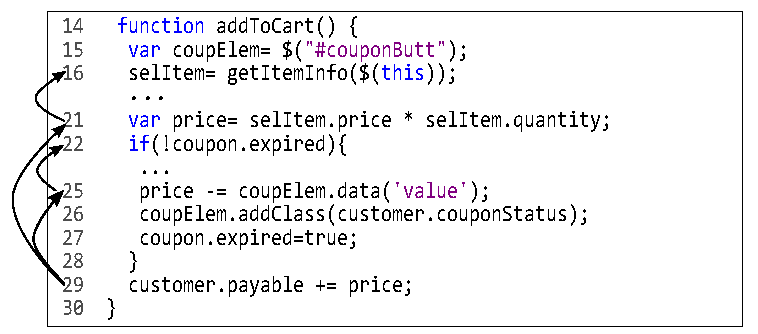
\includegraphics[width=1\hsize]{fig/intraCodeDep}
  \vspace{-0.2in} 
  \mycaption{Intra code dependency within the \javascript code.}
  \label{Fig:intraCodeDep}
%  \vspace{-0.1in} 
\end{figure}
To determine the initial point of contact between DOM and the underlying application's code, we first cross reference the DOM element as well as the property we are interested in with a set of DOM mutations obtained from the execution trace. The desired DOM element and its property are inferred from either the intra DOM assertion dependency or the candidate DOM properties as described in \secref{extractDomRelatedInfo}. Recall that our execution trace contains information about triggered events, event handlers, and DOM mutations caused by the events. Therefore, we can identify relevant events and invoked functions corresponding to a given DOM mutation.
For example, the collected execution trace in \figref{assertionToCode} contains information about the mutations of a \code{div} element with class \code{shopContainer}, which pertains to the DOM-based assertion.

To figure out where the mutation originated in our execution trace, we keep record of DOM accesses within the invoked functions. For each DOM access, we track \javascript lines of code that are responsible for updating the corresponding DOM element. Going back to our example in \figref{assertionToCode}, given that the textual property of the \code{div} element is extracted from the intra DOM assertion dependency, we identify line 37 in function \code{viewCart} as the initial point of contact responsible for changing the \code{text} of DOM element.

After inferring DOM mutant statements, we identify the \emph{intra code dependency} within the application's code.
%gather the entire set of \javascript statements responsible for mutating a given DOM element.
\begin{mydef}[Intra Code Dependency]
\label{def:intraCodeDep}  
An intra code dependency is defined as $<criterion, codeSts>$, where $criterion$ is a variable at the initial point of contact, and $codeSts$ is the set of statements that are either affected by or influence the $criterion$. 
\end{mydef}
To find the intra code dependency, we perform backward as well as forward slicing techniques by using $criterion$ as the slicing criterion.
\textsc{GetBWSlice} in lines  15 and 21 of \algref{algorithm} computes a backward slice with respect to assertion related DOM mutations, and candidate DOM property mutations respectively.
We use dynamic slicing to capture run-time dependencies accurately.
Note that instrumenting the entire application's code to perform dynamic slicing incurs high performance overheads. To avoid this, we first intercept the code sent from the server to the client, and then statically instrument only those statements that may affect a given DOM element.
To extract the subset of the code statements, we first find the \javascript closure scope which contains the definition of the variable in the initial slicing criteria. Then all references to the variable within the closure scope are found. Therefore, we can identify all locations in the code where the variable is updated, read, or a new alias is created. For each variable update/read related to the variable of the slicing criteria, we track the data dependencies for such an operation. The aforementioned steps are performed iteratively for each dependencies to collect the subset of code statements, which are instrumented for a given initial slicing criteria.
The instrumented code keeps track of all updates and accesses to all relevant data and control dependencies.   
Once the test case runs, we collect traces from the instrumented code. This trace is used to dynamically extract backward slicing as well as forward slicing statements. Note that in addition to backwards slicing which is later used to generate explicit assertions, we also use forwards slicing to generate our implicit assertions (\secref{implicitAssertions}).  

The backwards slicing technique starts by extracting instances of the initial slicing criteria from the trace. For each \textit{read} operations, the trace is traversed backwards to find the nearest related \textit{write} operation. Once found, the \textit{write} operation is added to the slice under construction. This process is repeated for all the data dependencies related to that write operation. A similar approach is taken for including control dependencies in the slice. 
Our slicing technique supports inter procedural slicing. For example, if a variable is assigned by the return value of a called function, the slicer recursively tracks the function and performs a backward slice on the statement returned by the called function.
%We track the following types of function calls during the slicing process: (1) Regular function calls e.g. \code{func()}, (2) Method calls e.g. \code{obj.func()}, (3) Constructors e.g. \code{new func()}, (4) Function handlers e.g. \code{element.click(func)}, and (5) Anonymous functions, which are assigned to a variable or an object property.
  
To address aliasing when computing the slice of a variable that has been set by a non-primitive value, we need to consider possible aliases that may refer to the same object. Specifically in \javascript \textit{dot notation} and \textit{bracket notation} are frequently used to modify objects at run time. Since static analysis techniques often ignore this issue \cite{Feldthaus:icse13}, we use dynamic slicing. If a reference to an object of interest is saved to a second object's property, e.g. through the use of the \textit{dot notation}, the object of interest may also be altered via aliases of the second object. For example, after executing statement \code{a.b.c = objOfInterest;}, updates to \code{objOfInterest} may be possible through \code{a}, \code{a.b}, or \code{a.b.c}. To deal with such scenarios, our slicing technique searches through the collected trace and adds the forward slice for each detected alias to the current slice for our variable of interest (e.g. \code{objOfInterest}). 

Given \code{customer.payable} as the initial slicing criteria in our example, \figref{intraCodeDep} shows the relevant backward slice statements (lines 29, 25, 22, 21, and 16), where \code{customer.payable},  variable \code{price}, as well as properties of the object \code{selItem} are assigned, and the value of \code{coupon.expired} is checked in the conditional statement.
By the end of backward slicing step, we collect all the relevant statements to a given DOM element. These are later used to derive test assertions.    